\documentclass{csse4400}

% \teachermodetrue

\usepackage{languages}

\title{Storing Stuff}
\author{Brae Webb}

\date{\week{3}}
\begin{document}

\maketitle

\begin{figure}[h]
  \href{https://www.oreilly.com/library/view/designing-data-intensive-applications/9781491903063/ch02.html}{
    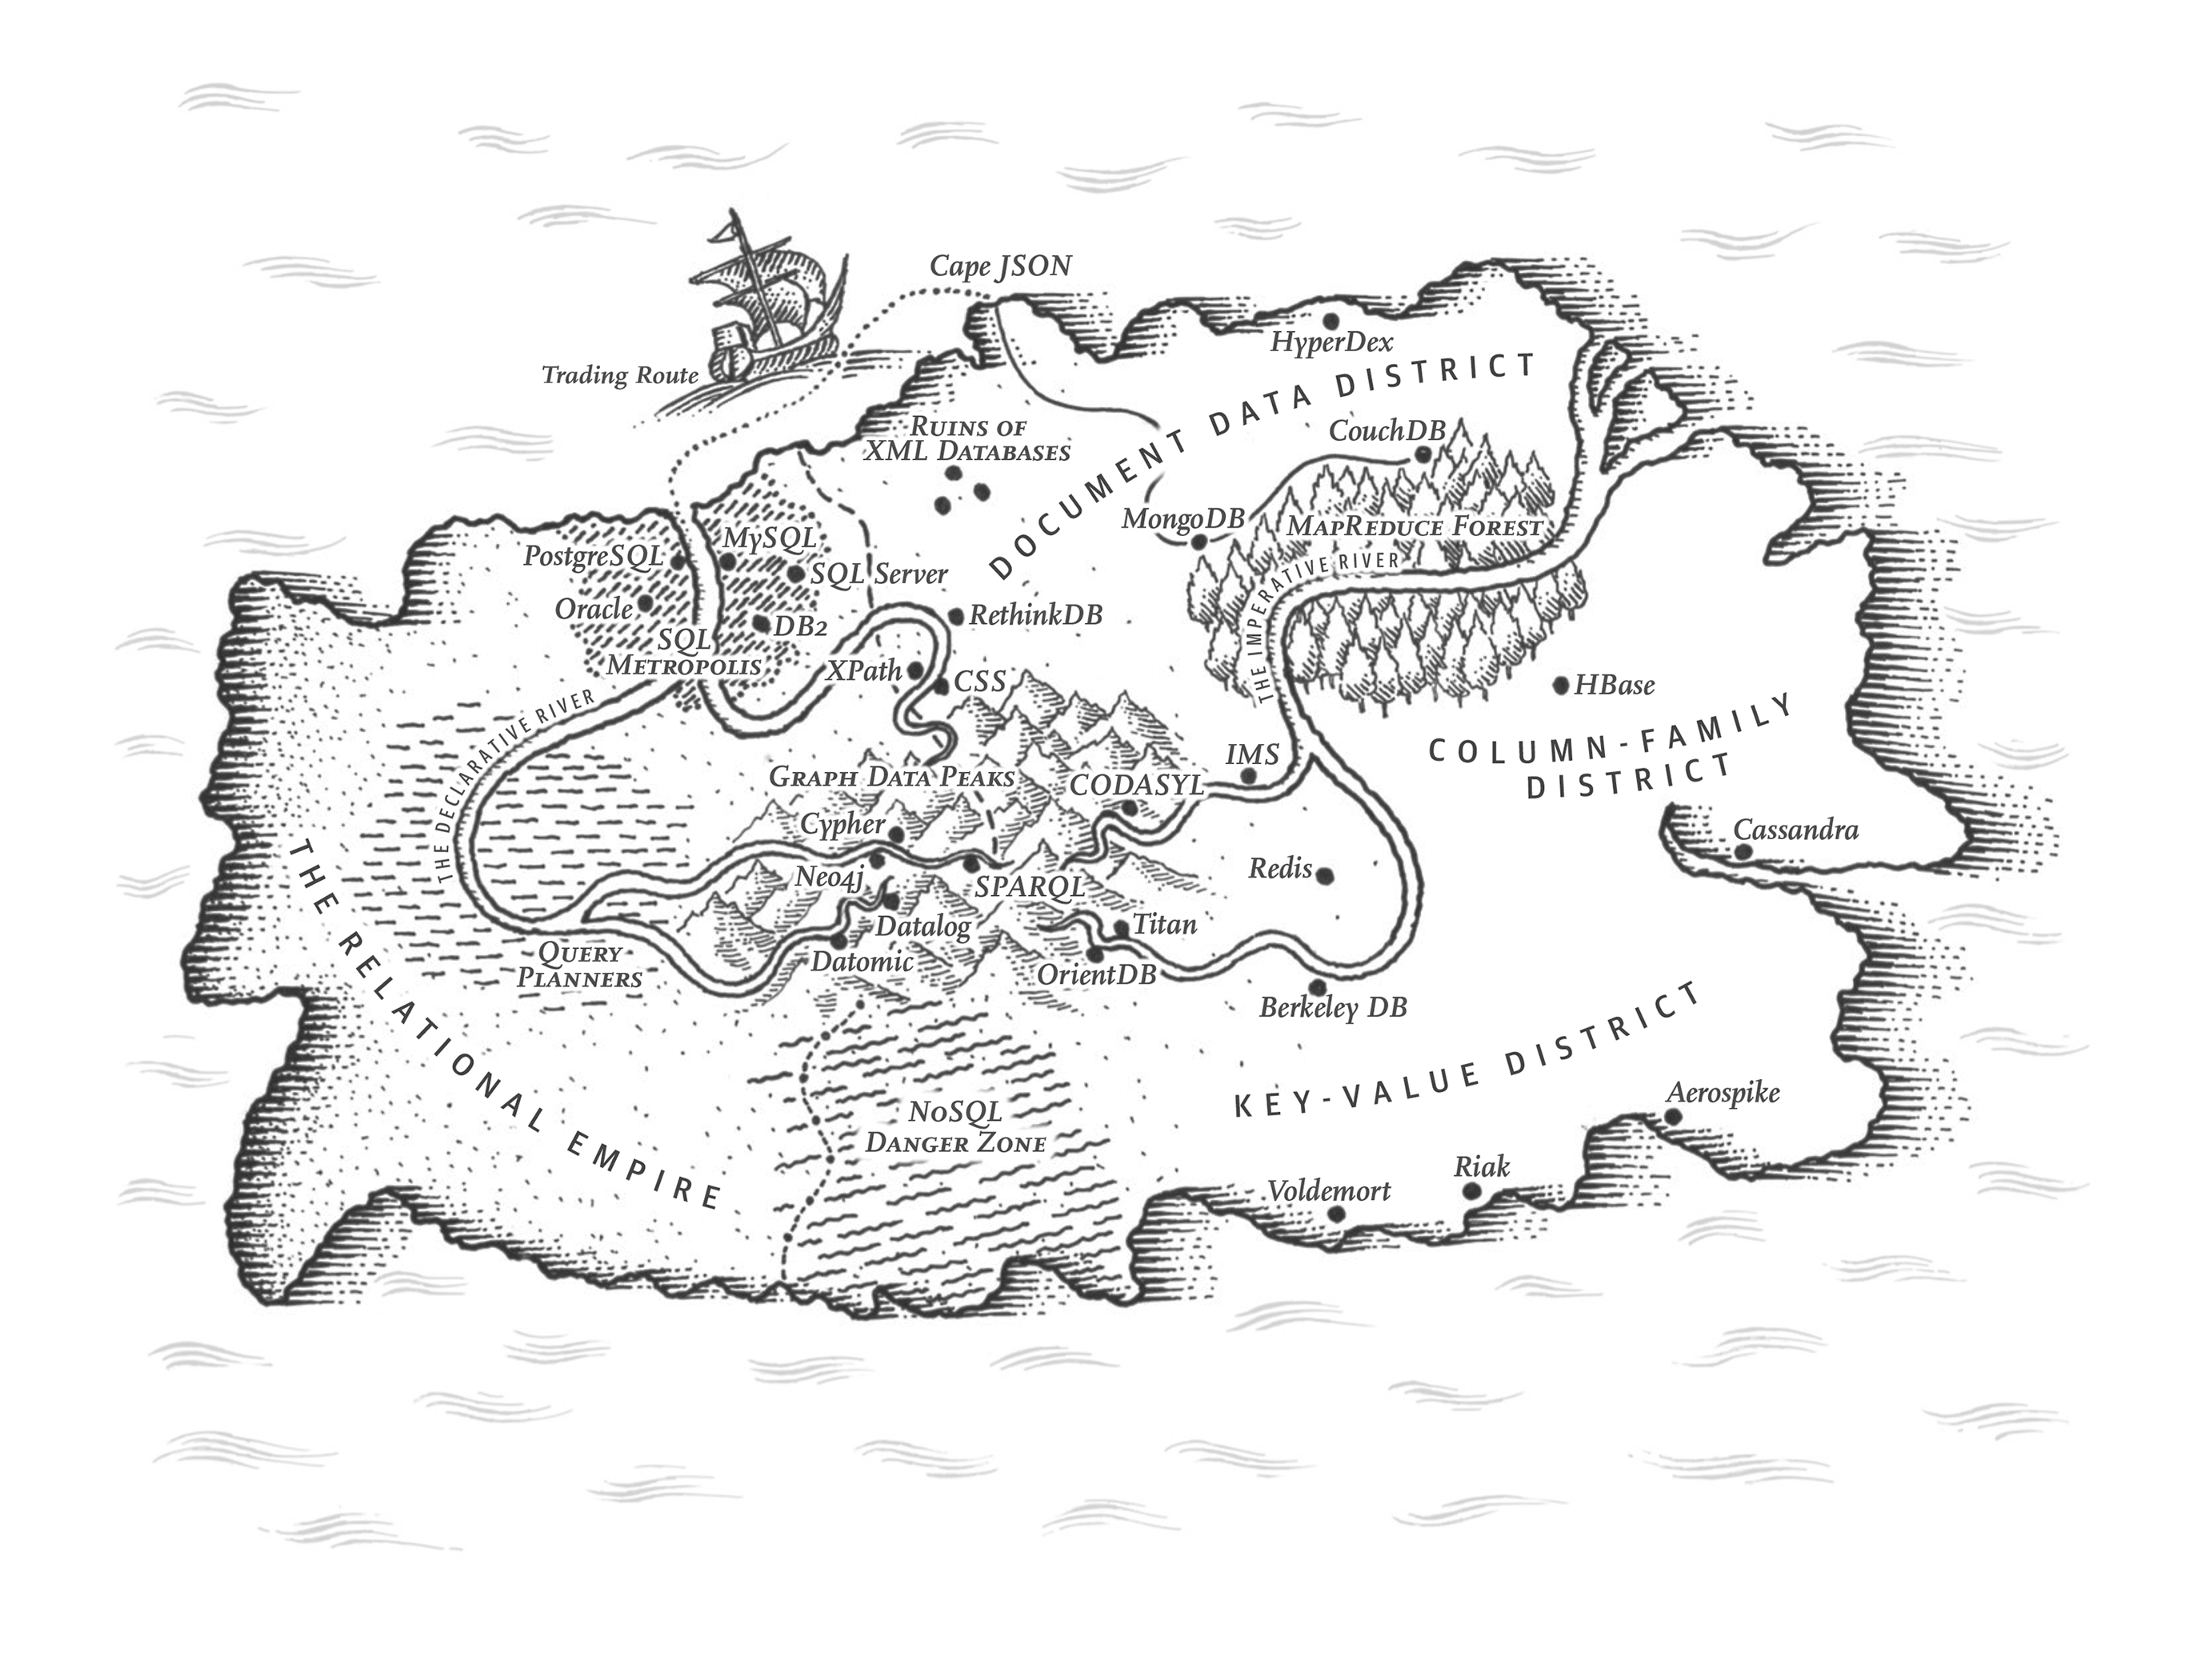
\includegraphics[width=\textwidth]{images/databases}
  }
\caption{A map of data storage techniques from Designing Data-Intensive Applications \cite{data-intensive}.}
\end{figure}

\section{This Week}
This week our goal is to:
\begin{itemize}
  \item explore the various techniques developers use to store data; and
  \item look at the storage options implementing these techniques on the AWS platform.
  \item run a small application using docker that requires a database.
  \item deploy a small application that requires a database in AWS using Terraform.
\end{itemize}

\section{Introduction}
Unfortunately, to build interesting software we often need to store and use data.
The storage of data introduces a number of challenges to designing, creating, and maintaining our software.
However, not all data storage techniques are created equal;
the choice of data storage model can have a profound impact on our software's complexity and maintainability.
In this practical, we want to take a superficial exploration our island of data storage models.
For a more in-depth treatment of data storage models that is outside the scope of this course,
see the \textit{Designing Data-Intensive Applications} book \cite{data-intensive}.

\section{Relational Storage}
\begin{itemize}
  \item MySQL/MariaDB [ Amazon RDS / Amazon Aurora ].
  \item Postgres [ Amazon RDS / Amazon Aurora ].
\end{itemize}

  \subsection{ORM}
  Just mentioning the relational-object mismatch.

\section{Wide-Column Storage}
  \begin{itemize}
    \item Apache Cassandra [ Amazon Keyspaces for Cassandra ].
    \item Apache HBase.
  \end{itemize}

\section{Key-Value Storage}
\begin{itemize}
  \item Redis [ Amazon ElastiCache for Redis ].
  \item Memcached [ Amazon ElastiCache for Memcached].
  \item Amazon DynamoDB.
  \item Amazon MemoryDB for Redis.
\end{itemize}

\section{Time Series Storage}
\begin{itemize}
  \item Amazon Timestream.
  \item TimescaleDB ( Postgres + Addon ).
  \item Prometheus.
\end{itemize}

\section{Document Storage}
\begin{itemize}
  \item MongoDB.
  \item Apache CouchDB.
  \item Amazon DocumentDB.
\end{itemize}

\section{Graph Storage}
\begin{itemize}
  \item Amazon Neptune.
  \item Neo4J.
  \item Janus Graph.
\end{itemize}

\section{Working with Docker}

So far in the course we have introduced docker as a means to package software to make it easier to work with and deploy.
Today we will be using it to run a small application locally that is a webserver + a database.

\info{
    You will need to have docker and docker-compose installed for this practical.
    Installation will depend on your operating system.

    \begin{itemize}
      \item docker compose: https://docs.docker.com/compose/install/
      \item docker engine: https://docs.docker.com/get-docker/
    \end{itemize}
    
    We also recommend installing the vscode docker plugin or the equlivant tools in IntelliJ IDEs.
}

\notice{
    For terminal examples in this section, lines that begin with a \$ indicate a line which you should 
    type while the other lines are example output that you should expect. Not all of the output is captured 
    in the examples to save on space.  
}

\subsection{Locally}

\begin{code}[language=docker]{Dockerfile}
FROM ubuntu:21.10
RUN apt-get update \
        && DEBIAN_FRONTEND=noninteractive apt install -y \
            php \
            php-mysql \
            php-xml \
            php-curl \
            curl \
            git \
            unzip
RUN curl -sS https://getcomposer.org/installer | php -- --install-dir=/usr/local/bin --filename=composer
COPY . /app
WORKDIR /app
RUN composer install
CMD ["php", "artisan", "serve", "--host=0.0.0.0"]
\end{code}

\todo{ .. write the docker compose file. }

\begin{code}[language=docker-compose]{main.tf}
version: '3.3'
services:
  backend:
    image: ghcr.io/csse6400/todo-app:latest
    restart: always
    ports:
      - '8000:8000'
    environment:
      APP_ENV: 'local'
      APP_KEY: 'base64:8PQEPYGlTm1t3aqWmlAw/ZPwCiIFvdXDBjk3mhsom/A='
      APP_DEBUG: 'true'
      LOG_LEVEL: 'debug'
\end{code}

\todo{Include photo showing that we couldnt connect to DB}

\begin{code}[language=docker-compose]{main.tf}
version: '3.3'
services:
  db:
    image: mysql:8-debian
    restart: always
    environment:
      MYSQL_DATABASE: 'todoapp'
      MYSQL_USER: 'todoapp'
      MYSQL_PASSWORD: 'password'
      MYSQL_ROOT_PASSWORD: 'password'
    ports:
      - '3306:3306'

  backend:
    image: ghcr.io/csse6400/todo-app:latest
    restart: always
    depends_on:
      - db
    ports:
      - '8000:8000'
    environment:
      APP_ENV: 'local'
      APP_KEY: 'base64:8PQEPYGlTm1t3aqWmlAw/ZPwCiIFvdXDBjk3mhsom/A='
      APP_DEBUG: 'true'
      LOG_LEVEL: 'debug'
      DB_CONNECTION: 'mysql'
      DB_HOST: 'db'
      DB_PORT: '3306'
      DB_DATABASE: 'todoapp'
      DB_USERNAME: 'todoapp'
      DB_PASSWORD: 'password'
\end{code}

\subsubsection{Optional Exercise: Fixing the container}

In a typical application you dont want to have to enable debug and access an endpoint which is broken inorder
to run the database migrations. One way for us to fix this is to run the database migrations when our application starts.
Luckily for us the application we have is based off of Laravel which has a cli which can do this for us.

\todo{
  Walk through building a new container with a script that runs the migrations first.
}

\subsection{AWS}

\todo{ .. write the terraform to deploy instead. }

\bibliographystyle{ieeetr}
\bibliography{books}

\end{document}